\documentclass[10pt]{beamer}
%\usetheme[
%%% option passed to the outer theme
%    progressstyle=fixedCircCnt,   % fixedCircCnt, movingCircCnt (moving is deault)
%]{}
  
% If you want to change the colors of the various elements in the theme, edit and uncomment the following lines

% Change the bar colors:
%\setbeamercolor{Feather}{fg=red!20,bg=red}

% Change the color of the structural elements:
%\setbeamercolor{structure}{fg=red}

% Change the frame title text color:
%\setbeamercolor{frametitle}{fg=blue}

% Change the normal text color background:
%\setbeamercolor{normal text}{fg=black,bg=gray!10}

%-------------------------------------------------------
% INCLUDE PACKAGES
%-------------------------------------------------------

\usepackage[utf8]{inputenc}
\usepackage{quoting}
\usepackage{tikz}
\usepackage{natbib}

%-------------------------------------------------------
% DEFFINING AND REDEFINING COMMANDS
%-------------------------------------------------------

\usetheme{Warsaw}

%-------------------------------------------------------
% INFORMATION IN THE TITLE PAGE
%-------------------------------------------------------

\title[] % [] is optional - is placed on the bottom of the sidebar on every slide
{ % is placed on the title page
      \textbf{Analysis of "Cloudlet-based Efficient Data Collection in Wireless Body Area Networks" report}
}

\subtitle[]
{
      \textbf{MSA 2019-2020}
}

\author[Andrea Graziani - 0273395]
{      Andrea Graziani - 0273395 \\
      {}
}

\institute[]
{
      Università degli Studi di Roma “Tor Vergata” \\
      FACOLTA' DI INGEGNERIA \\
      Corso di Laurea Magistrale in Ingegneria Informatica
  
  %there must be an empty line above this line - otherwise some unwanted space is added between the university and the country (I do not know why;( )
}

\date{\today}

%-------------------------------------------------------
% THE BODY OF THE PRESENTATION
%-------------------------------------------------------

\begin{document}

%-------------------------------------------------------
% THE TITLEPAGE
%-------------------------------------------------------

{% % this is the name of the PDF file for the background
\begin{frame}[plain,noframenumbering] % the plain option removes the header from the title page, noframenumbering removes the numbering of this frame only
  \titlepage % call the title page information from above
\end{frame}}

%---------------------------------------------------------------------------------------------------------%
\begin{frame} 
%---------------------------------------------------------------------------------------------------------%

\section{Introduction}

\vspace{0.3cm}

\begin{quoting}[font=itshape, begintext={``}, endtext={''\cite[par.~1.4]{MSAReport}}]
The main goal of this paper is to develop a large scale WBANs system in the presence of cloudlet-based data collection model. The objective is to minimize end-to-end packet cost by dynamically choosing data collection to the cloud by using cloudlet based system [...] reducing packet-to-cloud energy, the proposed work also attempt to minimize the end-to-end packet delay
\end{quoting}

\vspace{0.3cm}

According to \citet{MSAReport}, the goal of their work is to built an efficient \textbf{Wireless Body Area Networks} (\textbf{WBAN}) exploiting \textbf{edge computing}, a new paradigm in which substantial computing and storage resources, referred to as \textbf{cloudlets}, are placed at the \textbf{Internet's edge}, that is in close proximity to WBAN devices or sensors.

To be more precise, as stated by \citet{MSAReport}, edge computing resources are exploited in order to \textbf{minimize average power consumption} and \textbf{transmission delay} when \textbf{Personal Digital Assistant} (\textbf{PDA}) of any WBAN user transmits collected data.



How edge computing resources are been exploited by \citet{MSAReport} to achieve their objectives? 

%---------------------------------------------------------------------------------------------------------%
\end{frame} 
%---------------------------------------------------------------------------------------------------------%
\section{An Edge-Accelerated, Cloud-Native Application}
\subsection{The role of communication technology}
%---------------------------------------------------------------------------------------------------------%
\begin{frame}{The role of communication technology} 
%---------------------------------------------------------------------------------------------------------%

The research is based on the observation according to which using WiFi communication technology a WBAN user is able to transmit data packet to the enterprise cloud with \textbf{low power consumption}, \textbf{low delay} and mostly \textbf{no connection cost} compared with cellular communication technology. In fact, researchers wrote:

\vspace{0.3cm}

\begin{quoting}[font=itshape, begintext={``}, endtext={''\cite[par.~3.1]{MSAReport}}]
It was shown that, via WiFi, the transmission power of a data packet of size 46 Bytes will cost about 30 mw and with a delay of 0.045 ms. On the other hand, a longer transmission range cellular network connection (e.g. 3G and LTE) is capable of transmitting the data packet to the cloud from any location that is cover by cellular network, which is usually a wider geographic area compared with the WiFi. It was shown that, via cellular, the transmission power of data packet of size 46 Bytes will cost about 300 mw and with a delay of 0.45 ms.
\end{quoting}

\vspace{0.3cm}

%---------------------------------------------------------------------------------------------------------%
\end{frame} 
%---------------------------------------------------------------------------------------------------------%
\subsubsection{MAC protocol}
%---------------------------------------------------------------------------------------------------------%
\begin{frame}{MAC protocol} 
%---------------------------------------------------------------------------------------------------------%

\begin{itemize}

\item Medium access mechanisms used is \textbf{pooling-based}.

\item This choice has several advantages:

\begin{itemize}

\item is capable to offer time-bounded service, \textbf{guaranteeing a maximum access delay and minimum transmission bandwidth} making the system more \textbf{predictable} and, therefore, more suitable for \textbf{real-time} health monitoring.

\item Since WBAN users are not allowed to send data without the master's invitation, the \textbf{hidden terminal problem is eliminated}.

\item This scheme allow higher throughput due to less collisions respect to CSMA/CA.\cite{schiller2003mobile}

\end{itemize}

\end{itemize}

%---------------------------------------------------------------------------------------------------------%
\end{frame} 
%---------------------------------------------------------------------------------------------------------%
\subsection{The role of edge computing}
%---------------------------------------------------------------------------------------------------------%
\begin{frame}{The role of edge computing} 
%---------------------------------------------------------------------------------------------------------%

How to exploit WiFi technology in WBAN systems taking into account its \textbf{short transmission range} compared to cellular network? According to \citet{MSAReport}, the answer is \textit{providing an edge computing infrastructure made up of several cloudlet geographically distributed and equipped with computational, storage and communication capabilities}. Researchers wrote:

\vspace{0.3cm}

\begin{quoting}[font=itshape, begintext={``}, endtext={''\cite[par.~4.1]{MSAReport}}]
The cloudlet system is composed of set of physical servers with many cores and huge Gigabytes of memory. The cloudlet server system is equipped with one or more of the communication antennas that is supporting different physical layer capabilities (e.g. WiFi and WiMax). 
\end{quoting}

\vspace{0.3cm}

In other words, distributing geographically several cloudlets with aforementioned capabilities in a region, is possible to extend WiFi coverage increasing the probabilities that WBAN users use WiFi as communication technology. However, there are other reasons which induced researchers to adopt this solution. 

\citet{MSAReport} report that WBAN devices and sensors have very stringent constraints in term of CPU performance, storage resources and battery life. As also mentioned by the researchers, to perform a wide range application in a WBAN system, the so called \textbf{Tier-1}, which represents "\textit{the cloud}" in today's parlance, plays a very important role in this kind of system, because its resources are exploited to overcome WBAN devices constraints. Tier-1 represents, in terms of archival preservation, the \textit{safest place to store data}, ensuring the long-term integrity and accessibility, and the \textit{main execution site to perform expensive computations}, thanks to its almost unlimited elasticity. In fact, \citet{MSAReport} wrote that:

\vspace{0.3cm}

\begin{quoting}[font=itshape, begintext={``}, endtext={''\cite[par.~3.2]{MSAReport}}]
In our implementation, the enterprise cloud system will be the ultimate destination of the collected data. The enterprise cloud is also able to send messages back to both the cloudlet system or to WBAN users.
\end{quoting}

\vspace{0.3cm}

\begin{quoting}[font=itshape, begintext={``}, endtext={''\cite[par.~4.1]{MSAReport}}]
The enterprise cloud system is a centralized management and storage point that can be accessed by different organizations that are interested in a certain type of data. Another important feature of the cloudlet system is the ability of bidirectional communications between many WBANs users.
\end{quoting}

\vspace{0.3cm}

However cloud resources exploitation isn't a panacea due to some negative consequence, like an increasing of network \textbf{round-trip times} (\textbf{RTT}) experienced by mobile users, an \textbf{high ingress bandwidth}, \textbf{privacy issues} and \textbf{cloud outages}. To \textit{partially} overcome these problems, \citet{MSAReport} have built a system, capable to exploit edge computing resources, intended for so called \textit{edge-accelerated, cloud-native applications}. \cite{TheSeminalRoleEdgeNativeApplications}\cite{TheEmergenceOfEdgeComputing} In fact:

\begin{description}

\item[cloud-native] because, to overcome stringent constraints on battery, performance and storage of WBAN devices, cloud resources are exploited, through offloading techniques over a wireless network, \textbf{to execute critical task}; in other words, as stated also by \citet{MSAReport}, \textit{cloud is the primary execution site and it is essential to provide services to final users}.

\item[edge-accelerated] because the system exploits edge computing resources \textbf{only when available}. In that way, that system is capable to provide optimal performance, but \textit{edge resources represents a secondary execution site, that is they are optional to provide services}.

\end{description}

According to \citet{TheSeminalRoleEdgeNativeApplications}, it is shown that edge-accelerated, cloud-native applications can have a \textit{modest} advantages in term of \textit{response times}, \textit{battery life}, \textit{ingress bandwidth demand reduction}, \textit{privacy} and \textit{fallback services}\cite{TheSeminalRoleEdgeNativeApplications}\citep{TheEmergenceOfEdgeComputing}, because, as \citet{TheSeminalRoleEdgeNativeApplications} states, edge computing potentiality is not fully exploited due to central role assigned to cloud in this kind of system. However, respect to edge native application, it is true that any edge-accelerated, cloud-native applications involves less investment risk, much less software development, and their markets are much larger since they \textit{can function acceptably even in the absence of edge computing}.

Anyway, deploying cloudlet \textit{close} to final users, thanks to \textbf{high-bandwidth single-hop connection}, is possible to reduce RTT and to increase end-to-end bandwidth; in other words, we can achieve \textbf{network-proximity}.\citep{TheSeminalRoleEdgeNativeApplications}

However, is very important to not confuse \textit{physical proximity} with \textit{network-proximity}. Cloudlet physical proximity not always can affect positively RTT since it does \textit{not} guarantee network proximity: think for example to a highly congested WiFi network which may have poor RTT. Theoretically, is possible to achieve network proximity without physical proximity, for example using a fiber link between a wireless access point and a cloudlet that is many tens or even hundreds of kilometres away assuring therefore low RTT and high bandwidth.\cite{TheSeminalRoleEdgeNativeApplications}


%---------------------------------------------------------------------------------------------------------%
\end{frame} 
%---------------------------------------------------------------------------------------------------------%
\subsection{A self-adaptive system}
%---------------------------------------------------------------------------------------------------------%
\begin{frame}{A self-adaptive system} 
%---------------------------------------------------------------------------------------------------------%

Since WiFi technology transmission range is short and edge infrastructure resources are expensive, cloudlet and WiFi coverage aren't available everywhere. Therefore, \citet{MSAReport} implemented a \textit{self-adaptive behaviour} according to which \textbf{communication technology is dynamically changed} when users move from one region to another. This is the reason according to which \citet{MSAReport} have identified three different regions:\cite[par.~3.1]{MSAReport} 

\begin{description}

\item[Cloudlet Region (CR)] where WiFi coverage is available, so a user can use it to transmit data to the cloudlet.

\item[Enterprise Region (ER)] where only cellular coverage is available, therefore  a user can use only cellular technology to transmit a data packet to cloud. 

\item[Not-covered Region (NC)] where neither WiFi nor cellular technology is available. In this case a user should buffer the packets until one of the above technologies is available, then to be able of transmitting the packet to the enterprise cloud. 

\end{description}

In other words, WBAN users are capable to exploit edge computing resources if and only if they are in a \textit{Cloudlet Region}, otherwise they go on transmitting data directly to the cloud. In other words, \citet{MSAReport} have built a \textbf{self-adaptive} system because \textit{it is capable to change its behavior, changing communication technology, when execution environment changes, that is when change the region where a WBAN user is situated}. 

From a deployment point of view, this system represents a \textbf{distributed self-adaptive system} since a self-adaptive software, including both \textit{managed software} and \textit{managing software}, is deployed in every WBAN users device.\cite{PatternsDecentralizedSelf}

From decisions control point of view, we can consider it a \textbf{decentralized self-adaptive system} too due to the lack of a central control component that decides about when and how to perform an adaptation.\cite{PatternsDecentralizedSelf} 

However, is very important to precise that in \citet{MSAReport} system there is \textbf{no coordination} between WBAN nodes referring to control decision. All  of them act independently, deciding adaptations autonomously, therefore, \textit{any kind of control decisions decentralization pattern is been used}.  

From an architectural point of view, that system uses a \textbf{top-down approach} based on \textbf{MAPE-K feedback control loop}. Researchers wrote that:

\vspace{0.3cm}

\begin{quoting}[font=itshape, begintext={``}, endtext={''\cite[par.~5.1]{MSAReport}}]
each VC region is able to serve a certain number of users [...] Then, the extra users within the VCs have to send the data via the cellular communication, even though, they are within the VCs. 
\end{quoting}

\vspace{0.3cm}

In other words, \textit{WBAN devices exhibit a behavior according to which they can decide to offload towards cloud instead of cloudlet if Wifi network is highly congested}. This point is very important because an highly congested WiFi can lead to high latency, therefore, in accordance with policies established by \citet{MSAReport}, WBAN nodes  send data cellular communication, even though, they are within a cloudlet region.  

Therefore we believe that every WBAN node acts as an \textit{autonomic elements} because it manages their behavior in accordance not only with execution environmental changes, but according to \textit{policies and goals} established by \citet{MSAReport} too, in this case reducing transmission delay and power consumption. In other words, that system has \textbf{self-management capabilities}, relieving WBAN users of the responsibility of directly managing their device changing communication technology to achieve established goals; as known, self-management is the essence of \textbf{autonomic computing}.\cite{visionOf} 

Let's study in deep the control feedback loop of that system:
\begin{description}

\item[Knowledge/Goal] The goals established by \citet{MSAReport} are average power consumption and average transmission delay minimization.

\item[Monitor] The monitoring process is responsible for collecting data from environment like network quality and WiFi or cellular connection availability. 

\item[Analyse] Measured data are analysed in order to detect WiFi congestion condition level ("Low" or "High") and check what is the current region ("NC", "ER" or "CR") where user is.

\item[Plan] Select and plan a solution to achieve established goal in according to system state diagram represented in \ref{fig:Chain}. 

\item[Execute] Change communication technology according to current state.

\end{description}

Finally, \citet{MSAReport} solution can be considered as \textbf{application-transparent} since WBAN applications are \textit{not} informed that a communication technology change is occurred; in other words, underlying system is the only responsible for the adaptation. In this way, compatibility with already existing applications is assured, although adaptations can affect negatively on WBAN applications. 

\begin{figure}
\caption{State diagram of communication technology used by WBAN devices} \label{fig:Chain}
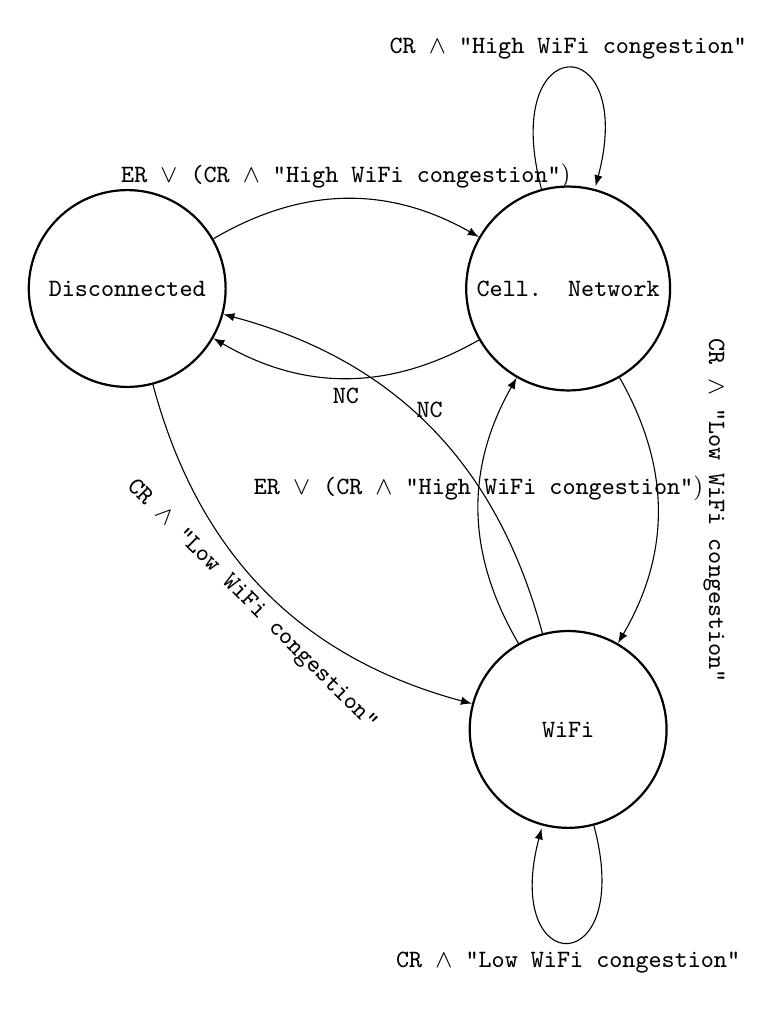
\begin{tikzpicture}[->,node distance=5.6cm,>=latex,font=\small, minimum width=2.5cm]

\tikzstyle{round}=[thick,draw=black,circle]

    \node[round] 			    		 (00) {\texttt{Disconnected}};
    \node[round,right of=00]      (10) {\texttt{Cell. Network}};
    \node[round,below of=10]    (01) {\texttt{WiFi}};

	\path 
 	(00) 	edge[bend left, above]        node	 	{\texttt{ER $\vee$ (CR $\wedge$ "High WiFi congestion"})} 							(10)
 	        edge[bend right, below]      node [rotate=-45]				    {\texttt{CR $\wedge$ "Low WiFi congestion"}} 							(01)
 	
	(10) edge[bend left, above]        node [xshift=13,rotate=-90]	{\texttt{CR $\wedge$ "Low WiFi congestion"}} 							(01)
		   edge[bend left, below]        node 	{\texttt{NC}} 																		(00)
		   edge[loop above]      		  node   {\texttt{CR $\wedge$ "High WiFi congestion"}} 							(10)
		   
	(01) edge[loop below]      		  node   {\texttt{CR $\wedge$ "Low WiFi congestion"}} 							(01)
		   edge[bend left, above]       	 node 	{\texttt{ER $\vee$ (CR $\wedge$ "High WiFi congestion"})} 						(10)
		edge[bend right, above]       	 node 	{\texttt{NC}} 						(00);

\end{tikzpicture}
\end{figure}

%---------------------------------------------------------------------------------------------------------%
\end{frame} 
%---------------------------------------------------------------------------------------------------------%
\subsection{The use of cyber-foraging techniques}
%---------------------------------------------------------------------------------------------------------%
\begin{frame}{The use of cyber-foraging techniques} 
%---------------------------------------------------------------------------------------------------------%

WBAN sensors and devices collect a very huge amount of data. In fact, \citet{MSAReport} wrote:

\vspace{0.3cm}

\begin{quoting}[font=itshape, begintext={``}, endtext={''\cite[par.~1.1]{MSAReport}}]
The multiple WBAN sensor nodes are capable of sampling, processing, and communicating one or more vital signs like heart rate, blood pressure, oxygen saturation, breathing rate, diabetes, body temperature, ECG and activity, or environmental parameters like location, temperature, humidity, light, movement, proximity and direction. 
\end{quoting}

\vspace{0.3cm}

Obliviously, WBAN devices cannot have enough computation and storage resources to manage that amount of data due to their very strictly constrains in term of size and power consumption. 

In order to overcome limitations of mobile devices used in WBAN, \citet{MSAReport} adopt several \textbf{cyber-foraging techniques} to exploit external resources to augment the computation and storage capabilities of WBAN devices extending their battery life. For instance, \textbf{computation offload tactic} is used to achieve energy-efficiency  increasing computing power, because all computations regarding collected data are carried out by cloud or cloudlet. 

\citet{MSAReport} have adopted \textbf{data staging} tactic too in order to improve WBAN applications performances managing \textbf{field-collected data}. In fact, when a WBAN application complete all its data collection operations, following situations may happen:

\begin{itemize}
\item If a WBAN user is close to a cloudlet, WBAN devices offload data to cloudlet and, when the operation is complete, they delete transmitted data to free up storage space. In addition, cloudlet forwards to enterprise cloud all data that was collected by the multiple users.

\item If a WBAN user cannot establish a connection with a cloudlet and a cellular data connection is available, all collected data will be offloaded directly to the cloud.
\end{itemize}

In other words, is clear that external resources are located in both \textbf{single-hop} and \textbf{multi-hop} proximity of the mobile devices that use them. In fact, when collected data are offloaded to a remote resource, that is enterprise cloud, \textbf{synchronous operations with multiple network hops} between the mobile device and the cloud are involved while, when data are offloaded to cloudlet, a \textbf{single-hop connection} is involved (although is not clear if cloudlet need to be connected at runtime to cloud or not).

Finally \citet{MSAReport} adopt a very static approach about offloading operations because, if a offload target is available, data will be \textbf{always} offloaded. This decision can lead to a negative consequence: previously we have said that WBAN devices can decide to offload towards cloud instead of clodulet even though they are within a cloudlet region. In this particular situation \textbf{cyber-foraging techniques can also lead to reduce resource efficiency} because, even though executing the expensive computation on a surrogate leads to energy efficiency, \textit{changing network conditions might cause greater resource consumption}: if a WBAN node detects that WiFi network conditions are bad and decide to use cellular network, inevitably more energy will be consumed increasing transmission delay.

%---------------------------------------------------------------------------------------------------------%
\end{frame} 
%---------------------------------------------------------------------------------------------------------%
\subsubsection{The cloudlet discovery and provisioning issue}
%---------------------------------------------------------------------------------------------------------%
\begin{frame}{The cloudlet discovery and provisioning issue} 
%---------------------------------------------------------------------------------------------------------%

We believe that the cyber-foraging system built by \citet{MSAReport} is too simple to achieve research's goals, because it lacks of some very important features. In fact, it is shown that cyber-foraging systems have \textit{at a minimum} the following combination of functional requirements \cite{DecisionModel}:

\begin{itemize}

\item  A need for computation offload, data staging, or both.
\item  A need to \textbf{provision a surrogate} with the offloaded computation or data staging capabilities.
\item  A need for the mobile device to \textbf{locate a surrogate} at runtime.

\end{itemize}

%---------------------------------------------------------------------------------------------------------%
\end{frame} 
%---------------------------------------------------------------------------------------------------------%
%---------------------------------------------------------------------------------------------------------%
\begin{frame}{The cloudlet discovery and provisioning issue} 
%---------------------------------------------------------------------------------------------------------%

\begin{itemize}

\item Although WBAN users \textit{need} to be able to locate available cloudlet in an area where stage data, \textbf{cloudlet discovery} issue has \textit{not} been addressed by \citet{MSAReport} in any way; we believe that it is a very big mistake because cloudlet discovery affects negatively energy consumption and response time and, anyway, it is a \textbf{functional requirements} for any cyber-foraging systems. 

Moreover, when you want to offload data or computation to a cloudlet, generally a \textbf{selection algorithm} to select best cloudlet is run. In WBAN systems, maximize energy efficiency, in order to preserve devices lifetime, is critical, therefore is preferable not run selection algorithm on WBAN devices, which can decrease energy efficiency (depending on the complexity of the algorithm and the number of monitored variables). Probably, using cloud surrogate directory tactic, according to which selection algorithms run on the cloud, is possible to improve WBAN lifetime. \cite{DecisionModel}

\item In the same way, \textbf{surrogate provisioning} is another functional requirements for any cyber-foraging systems which is not addressed by \citet{MSAReport}, therefore is not clear how cloudlets manage offloaded computation and/or data processing operations.

We will see later that \citet{MSAReport} had shown that packet process delay is affected by the number of virtual machine deployed in cloudlet. However, provisioning tactic affects this process delay too. It is shown that \textit{pre-provisioned cloudlet tactic} have the advantage of shorter provisioning times because the capabilities already reside on cloudlet, providing shorter response times to requests from mobile devices.\cite{DecisionModel}

\end{itemize}


%---------------------------------------------------------------------------------------------------------%
\end{frame} 
%---------------------------------------------------------------------------------------------------------%
\subsection{Communication style}
%---------------------------------------------------------------------------------------------------------%
\begin{frame}{Communication style} 
%---------------------------------------------------------------------------------------------------------%

\begin{itemize}

\item When a device cannot transfer data packet to cloudlet for some reason, WBAN users are obliged to communicate directly with server-side application running on cloud, therefore a classical \textbf{client-server style communication} is adopted, which use classic \textit{point-to-point} and \textit{synchronous} communications.

\item When a WBAN user is capable to communicate through a server, the system adopts a \textbf{loose-connector} communication style: \textbf{server-side client/agent/server model}. In that case, the \textit{agent} is the cloudlet, which, acting as a surrogate to perform cyber-foraging tactics, is located on the so-called "\textit{fixed}" side portion of the network and, precisely, on the edge of the network. 

\end{itemize}

%---------------------------------------------------------------------------------------------------------%
\end{frame} 
%---------------------------------------------------------------------------------------------------------%

\section{Simulations Analysis}
\subsection{First experiment set}

%---------------------------------------------------------------------------------------------------------%
\begin{frame}{First experiment set}
%---------------------------------------------------------------------------------------------------------%


First experiment set goal is to quantify both \textbf{packet process delay} and \textbf{power consumption}, due to packet computation, by cloudlet varying following system parameter.

\begin{enumerate}

\item number of virtual machine deployed on a cloudlet (0, 2, 4 or 8). The maximum number of deployable virtual machines is bounded by the number of physical processors available on cloudlet (\citet{MSAReport} prototype cloudlet have 8 physical processors, therefore 8 is the maximum number of deployable VMs).
 
\item processing speed of data packet, from a minimum 100 to a maximum of 900 \textbf{million instructions per second} (MIPS).

\item number of WBAN users (up to 150 users).

\end{enumerate}


%---------------------------------------------------------------------------------------------------------%
\end{frame} 
%---------------------------------------------------------------------------------------------------------%
%---------------------------------------------------------------------------------------------------------%
\begin{frame}{First experiment set: Results}
%---------------------------------------------------------------------------------------------------------%

\begin{itemize}

\item \textbf{Increasing the number of virtual machines running on a cloudlet, packet process delay will be reduced.}

It is shown that, if data packets can be processed in \textbf{parallel}, the \textbf{blocked time} can be reduced. In fact, fixed data packet \textit{average arrival rate} $\lambda$ and \textit{average service rate} $\mu$ of each virtual machine, system cloudlet \textbf{utilization}, that is \textit{the fraction of time according to which cloudlet is busy}, is reduced; each virtual machine, by symmetry, sees an arrival rate of $\dfrac{\lambda}{k}$, where $k$ is the number of deployed virtual machines. Therefore cloudlet utilization, which is equal to $\dfrac{\lambda}{k\mu}$, decrease increasing $k$. It is shown that, decreasing utilization, \textbf{blocked time} decreases.\cite{BassSoftwareArchitecture2003}

\end{itemize}

%---------------------------------------------------------------------------------------------------------%
\end{frame} 
%---------------------------------------------------------------------------------------------------------%
%---------------------------------------------------------------------------------------------------------%
\begin{frame}{First experiment set: Results}
%---------------------------------------------------------------------------------------------------------%

\begin{itemize}

\item \textbf{Fixed the average time required to process a packet data on a CPU, that is for a given MIPS process speed, power consumption and processing delay are increased by increasing the number of users.} 

This happens because cloudlet utilization increases because $\lambda$ is higher, therefore the fraction of time according to which cloudlet is busy increases too; so, since more time is needed to complete user tasks, more power is consumed.

\end{itemize}

%---------------------------------------------------------------------------------------------------------%
\end{frame} 
%---------------------------------------------------------------------------------------------------------%
\subsection{Second experiment set}
%---------------------------------------------------------------------------------------------------------%
\begin{frame}{Second experiment set} 
%---------------------------------------------------------------------------------------------------------%

Second experiment set was carried out in order to quantify advantages of using edge computing resources. To be more precise, that simulation monitors the effects on \textbf{average transmission power and delay} of data packed send by users PDA to cloudlet, varying following system parameters:

\begin{enumerate}
\item number of cloudlet deployed (from 0 to 6).
\item number of WBAN users (set to be 400, 600, 800, 1000, 1200 and 1400).
\end{enumerate}

Monitored area size is fixed to $600 \times 400\;m$.

%---------------------------------------------------------------------------------------------------------%
\end{frame} 
%---------------------------------------------------------------------------------------------------------%
%---------------------------------------------------------------------------------------------------------%
\begin{frame}{Second experiment set: Results}  
%---------------------------------------------------------------------------------------------------------%

\begin{itemize}

\item As expected, increasing the number of available cloudlets in monitored area, average transmission delay of data packed is reduced. It happens since the probability  that an user is close to one of them increases. Having more opportunities to transmit data within cloudlet coverage, users can benefit of \textit{cloudlet network proximity}. 

In fact, when cloudlet coverage is available, data is offloaded to a cloudlet using a high bandwidth single-hop connection, which decrease RTT. Conversely, when cloudlet coverage isn't available, data is offloaded to cloud using a multi-hop network connections which involves high RTT and likely low bandwidth connection.\cite{ArchitecturalTacticsCyberForaging}

\end{itemize}

%---------------------------------------------------------------------------------------------------------%
\end{frame} 
%---------------------------------------------------------------------------------------------------------%
%---------------------------------------------------------------------------------------------------------%
\begin{frame}{Second experiment set: Results} 
%---------------------------------------------------------------------------------------------------------%

\begin{itemize}

\item Increasing the number of available cloudlets, average transmission power of data packed is reduced too. It is due to the use of WiFi technology which is, as already said, more energy-efficient compared to cellular network.

\end{itemize}

%---------------------------------------------------------------------------------------------------------%
\end{frame} 
%---------------------------------------------------------------------------------------------------------%
%---------------------------------------------------------------------------------------------------------%
\begin{frame}{Second experiment set: Results} 
%---------------------------------------------------------------------------------------------------------%

\begin{itemize}

\item Increasing the number of users, both average transmission power and delay increase. This happens because:

\begin{enumerate}
\item When a cloudlet area contains a large number of users, interferences increase, leading to higher error bit rate and affecting negatively both transmission delay, due to data packets or acknowledgements loss, and power, due to packet retransmission.

\item Since a polling MAC scheme is used, an higher number of users within an cloudlet WiFi coverage area increases the time needed to pool every node by AP. 

\item As stated by \citet{MSAReport}, an high congested WiFi network can cause WBAN devices to perform a self-adaptation action according to which communication technology is switched, using cellular network to send packet data instead WiFi, affecting negatively aforementioned metrics.
\end{enumerate}

\end{itemize}

%---------------------------------------------------------------------------------------------------------%
\end{frame} 
%---------------------------------------------------------------------------------------------------------%
\subsection{Third experiment set}
%---------------------------------------------------------------------------------------------------------%
\begin{frame}{Third experiment set}
%---------------------------------------------------------------------------------------------------------%

The last experiment set is focusing on monitoring aforementioned performance metric varying cloudlet geographical placement. Monitoring an $800 \times 800 \; m$ area, simulations were carried out varying following system parameters:

\begin{enumerate}
\item number of cloudlet deployed (up to 16 cloudlets).
\item number of WBAN users (up to 1400 users).
\item WBAN user's positions (same parameters as before)
\item cloudlet geographical placement (using very different patterns, classified in three categories by \citet{MSAReport}: \textit{Adjacent}, \textit{Distant} and \textit{Intermediate})
\end{enumerate}

%---------------------------------------------------------------------------------------------------------%
\end{frame} 
%---------------------------------------------------------------------------------------------------------%
%---------------------------------------------------------------------------------------------------------%
\begin{frame}{Third experiment set: Results}
%---------------------------------------------------------------------------------------------------------%

Experiments results are the following:

\begin{itemize}

\item As expected, independently from cloudlet deployment pattern, increasing the number of cloudlet, the impact of cloudlet geographical placement on average transmission power and delay is negligible since, in that way, the opportunities to send the data packet to a cloudlet, using WiFi and with minimum cost of power and delay, increase.

\item Fixed cloudlet and users number, deploying cloudlet using an intermediate category pattern, that is placing cloudlet neither too far apart nor too close, system performance are better than other patterns belonging to other categories.

\end{itemize}

%---------------------------------------------------------------------------------------------------------%
\end{frame} 
%---------------------------------------------------------------------------------------------------------%
\section{Further considerations and possible improvements}
\subsection{IEEE 802.11ah as communication standard}
%---------------------------------------------------------------------------------------------------------%
\begin{frame}{IEEE 802.11ah as communication standard}
%---------------------------------------------------------------------------------------------------------%

In addition to changing communication technology, we believe that the use of a communication standard capable to minimize the main sources of energy waste like \textit{collision}, \textit{inter-network interference}, \textit{idle listening} and \textit{control packet overhead} is extremely useful to maximizing the lifetime of WBAN devices.

Unfortunately, \citet{MSAReport} give us very few details about MAC protocol, however is reasonable to assume that they have used legacy IEEE 802.11 protocol with $2.4$ or $5$ GHz bands.

We believe that we can achieve better communication performances over longer distances among a large number of low-power devices exploiting \textbf{IEEE 802.11ah}. In fact:

\begin{itemize}
\item The 802.11ah standard enables single-hop communication over distances up to $1000$ m, utilizing sub-1 GHz license-exempt bands to provide better propagation characteristics in outdoor scenarios, like WBAN, than legacy WiFi. On the other side

\item IEEE 802.11ah MAC layer improves power efficiency through frame shortening techniques, reducing overhead caused by short packets transmission which are very common in WBAN scenario.

\item Several innovative concepts such as hierarchical \textit{Association IDentification} (AID), \textit{Restricted Access Window} (RAW), \textit{Group Sectorization} (GS), decrease collision probability in networks with thousands of stations, resolve hidden terminal problems, support a large number of associated stations, improving scalability and power efficiency.

\end{itemize}

\subsection{Resource demand tactics}

In order to reduce system utilization, therefore reducing average packet process delay, we can adopt a particular \textbf{performance tactic}, called \textbf{resource demand tactics} according to which the number of packet to process can be reduced \textbf{managing the packets data generation rate}. In other words, if it is possible to reduce the sampling frequency at which environmental and body variables are monitored, demand can be reduced.\cite{BassSoftwareArchitecture2003} 

For instance, a possible solution suitable for WBAN could be to implement a self-adaptive behavior according to which sampling frequency can be temporary reduced when users population within a cloudlet region grows beyond a certain threshold.


\subsection{Variable data fidelity tactic}

Unfortunately \citet{MSAReport} \textit{didn't introduce any variable data fidelity tactic} capable to improve WBAN battery life. We believe that the introduction of an \textbf{approximate computing} (and \textbf{storage}) technique can be useful in WBAN context. 

As known, approximate computing is a new paradigm based on the intuitive observation that, while performing exact computation require high amount of resources, allowing selective approximation or imperfect computations results can provide drastic energy savings.

To be more precise, approximate computing leverage the presence of error-tolerant code regions in applications and perceptual limitations of users to intelligently trade off implementation, storage and/or result accuracy for performance or energy gains. In brief, approximate computing exploits the gap between the level of accuracy required by the applications/users and that provided by the computing system.

For example, can be useful, in order to improve energy-efficiency, to reduce data fidelity collected by WBAN devices according to network condition, current position or battery status. For instance, we can adopt a technique according to which, when network condition are very bad or totally absent, in order to reduce the energy cost due to data buffering, critical application data (for example vital signs like heart rate, blood pressure, oxygen etc.) are stored in reliable memory segments with higher refresh rate, conversely less critical data (for example experimental data like location, temperature, humidity, light etc.) are stored into less reliable memory with a less refresh rate. As known, higher is refresh rate, higher is power consumption.\cite{Towards}

\citet{ApproximateComputingArticle} had shown that, using approximate computing techniques, applications run 3.78 times faster while energy consumption are reduced 2.77 times.

\subsection{Scalability and elasticity tactic}

Solution proposed by \citet{MSAReport} doesn't exploit any scalability/elasticity tactic in order to increase cloudlet resource efficiency achieving scalability and elasticity. Keep running several virtual machines on a cloudlet while there are few WBAN users within a cloudlet region is a real waste of resources. Moreover full virtualization approaches are usually unsuitable for deploying distributed applications due to their overhead and long boot time.

OS-level virtualization based tools, also called \textbf{containers}, are often a better choice for scalability and elasticity purposes since they represent a lightweight alternative to virtual machine thanks to their very small footprint and quick boot time. 

Exploiting container advantages and using a scalability/elasticity tactic like \textbf{Just-in-Time containers tactic}, typically used to complement the computation offload tactic and data staging tactics, we can achieve aforementioned objectives. This tactic, in order to decrease the load on a cloudlet, supporting a greater number of requests, creates an instance of the offloaded code upon receipt of an offload request, destroying it when request is fulfilled. However, because the instance is created at runtime, there is a response/execution time penalty to create the instance before computation can execute.\cite{DecisionModel}\cite{ArchitecturalTacticsCyberForaging}

\subsection{Some considerations about mobility}

Due to WBAN users mobility, mobile devices may lose connectivity to cloudlet or cloud during offloading process. 

This situation can lead to an \textbf{high amount of disconnections} and consequently an \textbf{high amount of packet loss}, affecting negatively both power consumption and transmission delay; in fact, when wireless communication technologies are used, where many data packet can be lost due both to an \textit{high error bit rate} and to an \textit{high amount of disconnections}, TCP, one of the most important transportation protocol, interpreters packet loss as a congestion symptom, activating several congestion control mechanisms which, as known, negatively affect performance.\cite{tcp}

Although \citet{MSAReport} don't specify which transportation protocol is been used, we believe that the lack of focus about transportation protocol can be a big mistake due to aforementioned reasons. Since regular TCP was not designed with mobile hosts in mind, the use of a transportation protocol more suitable for wireless environment (like I-TCP, M-TCP, AIRMAIL etc.) can improve overall performances.

As known, when any WBAN user moves from a region to another, an hand-offs occurs, causing disconnections, data packets loss and performance worsening. Unfortunately, any information is given about \textit{average residence time} within a region by a WBAN user and the amount of hand-off performed during simulations. According to \citet{MSAReport}, WiFi coverage is limited to $100\;m$ which is very little if compared to cellular network transmission range. We believe that this situation could potentially lead to frequent hand-off and low residence time affecting negativity real applications.

\citet{MSAReport} doesn't report how \textit{users movements speed} (fixed to $2 m/s$) and the \textit{random pause time} (fixed to $1-10 s$) affected simulation's results and is not clear how they are intercorrelated with average power consumption and delay during the second and the third experiment set. Obliviously, we will expect that user speed is correlated to the amount of hand-off, therefore faster users involve more hand-offs, however this aspect was not considered. Moreover, we believe that \textbf{cloudlet region size} is a very important parameter since smaller cloudlet regions can potentially increase the amount of hand-off performed by an user.\cite{tcp} This aspect was also not considered.

Maybe, a better analysis regarding about aforementioned aspects, with a highlight system state variable describing how the state variables are interrelated, including algorithms for computing their interaction and evolution in time, would have been useful for reproducibility purposes, in order to  validate \citet{MSAReport} results.


\end{frame}



% ************************************************************************** %

\begin{frame}[plain,noframenumbering]
  Grazie per l'attenzione!
\end{frame}
\bibliography{Bibliography.bib}


\end{document}